\section{Примеры построенных множеств достижимости}

Приведем примеры для разного параметра $\alpha$. На рисунках приведена эволюция множества достижимости, а также траектории, удовлетворяющие теореме \ref{th:pmp} для наибольшего времени. Наибольшее время выбиралось таким, чтобы траектории системы могли быть посчитаны функцией \texttt{ode45}, то есть траектории не очень далеко от нуля.

\begin{figure}[h]
        \centering
        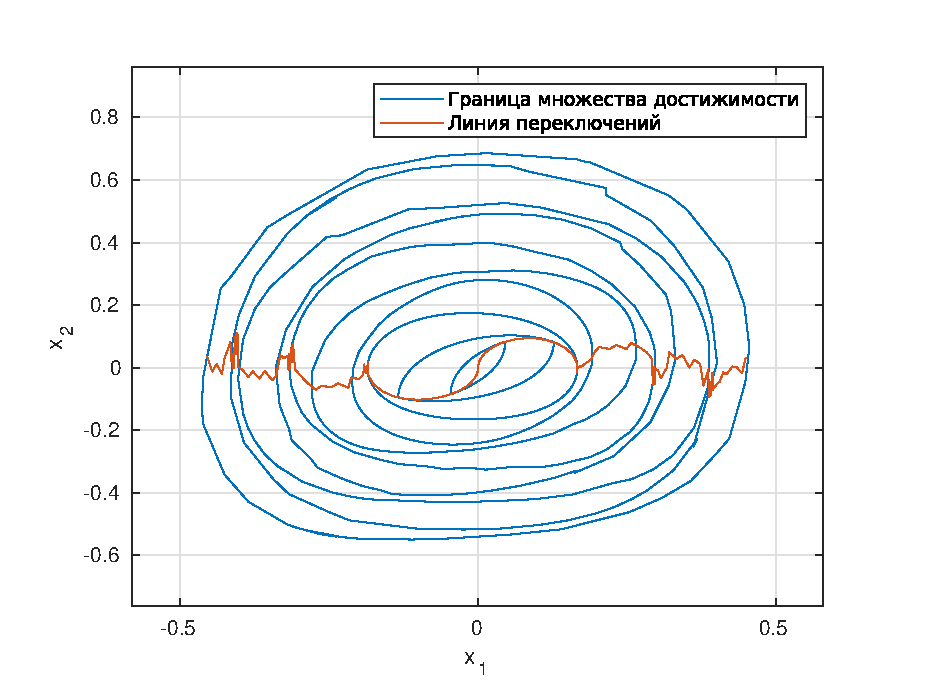
\includegraphics[width=0.49\linewidth]{examples/ev-start1end10alpha0-1.eps}
        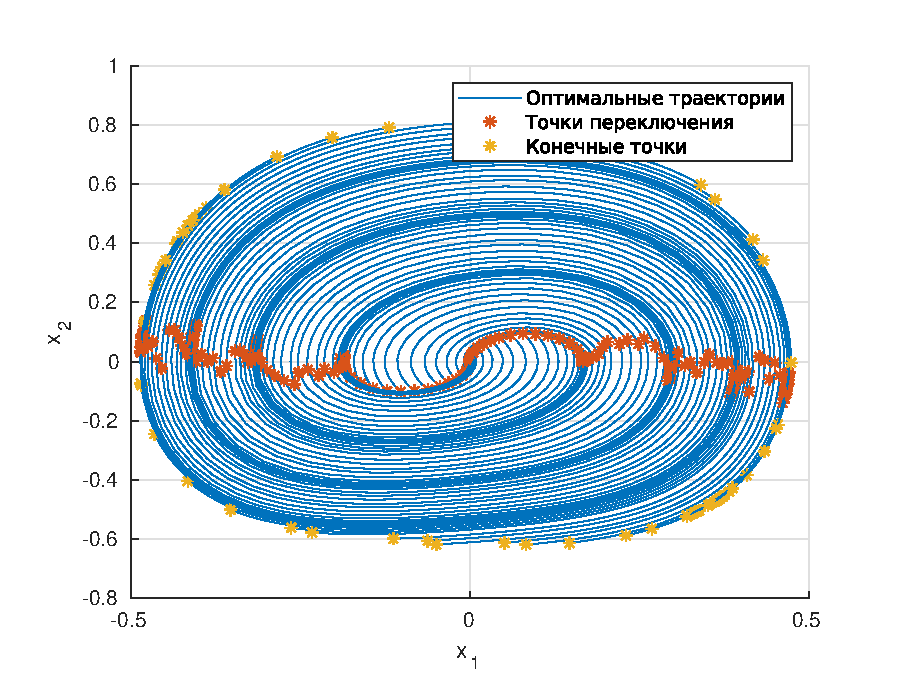
\includegraphics[width=0.49\linewidth]{examples/3.eps}
        \caption{$\alpha = \frac{1}{10}$, $t_1 = 1$, $t_2 = 10$.}
\end{figure}
\begin{figure}[h]
        \centering
        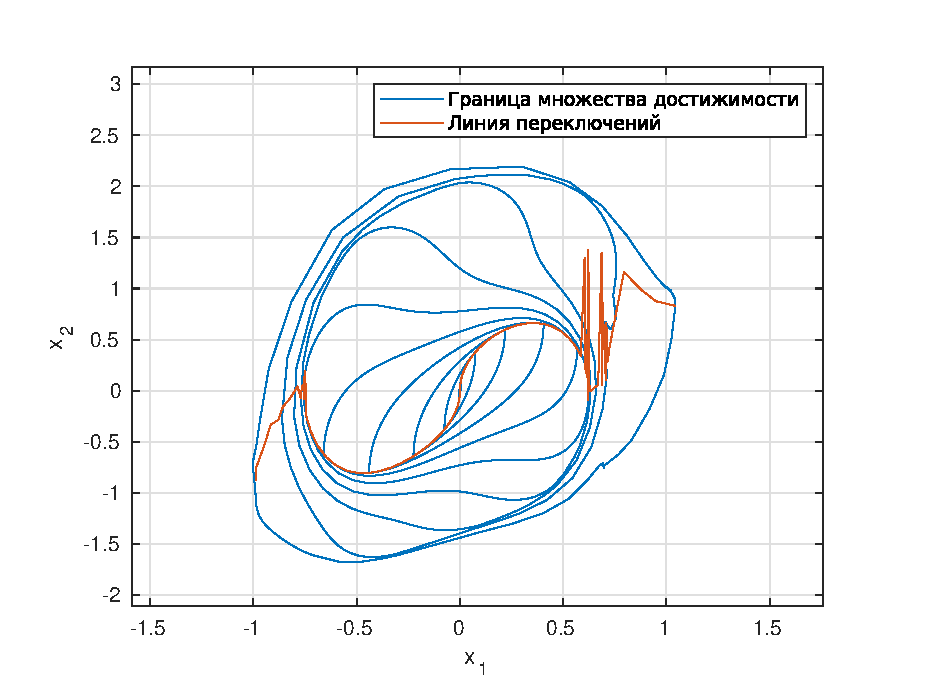
\includegraphics[width=0.49\linewidth]{examples/ev-start0-1end3alpha1.eps}
        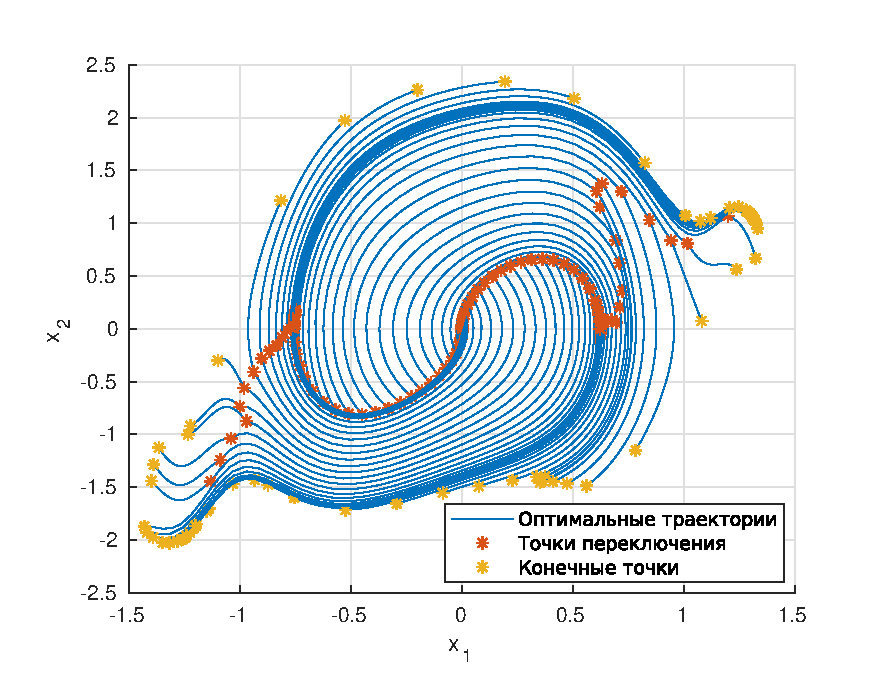
\includegraphics[width=0.49\linewidth]{examples/2.eps}
        \caption{$\alpha = 1$, $t_1 = \frac{1}{10}$, $t_2 = 3$.}
\end{figure}
\begin{figure}[h]
        \centering
        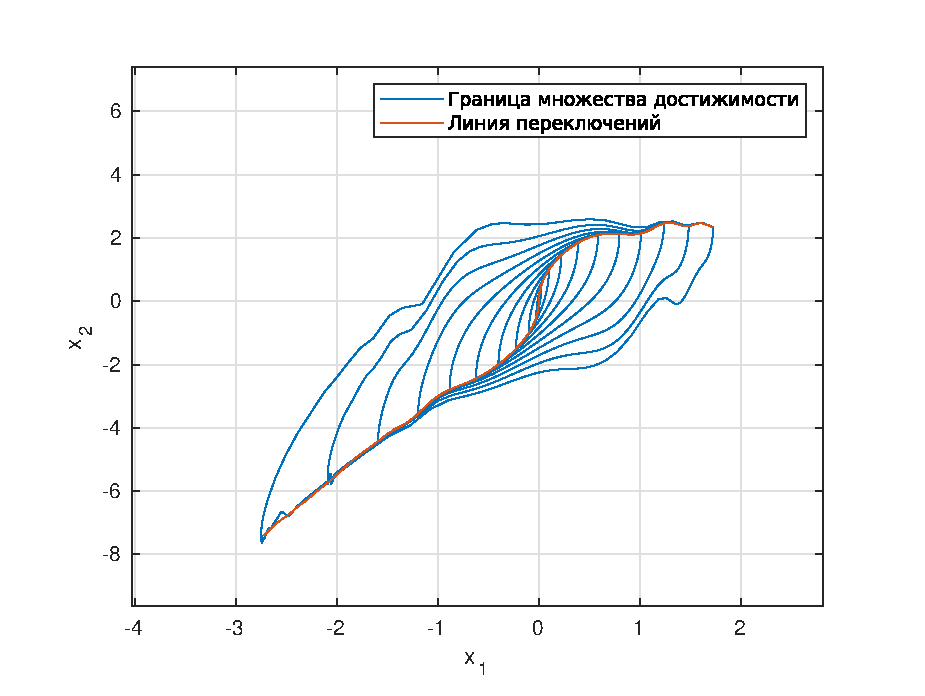
\includegraphics[width=0.49\linewidth]{examples/ev-start0-1end1alpha5.eps}
        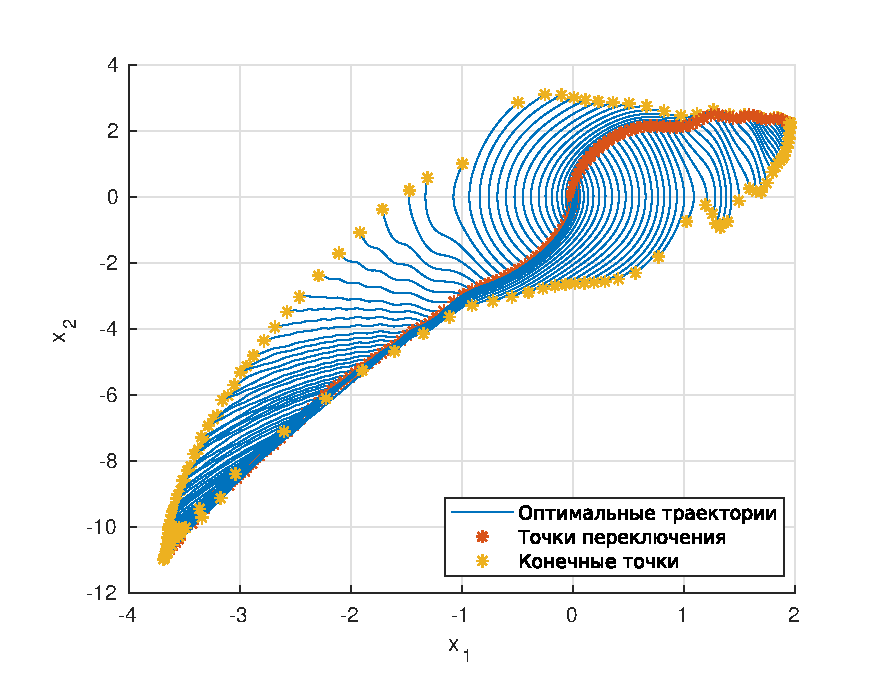
\includegraphics[width=0.49\linewidth]{examples/1.eps}
        \caption{$\alpha = 5$, $t_1 = \frac{1}{10}$, $t_2 = 1$.}
\end{figure}